\documentclass[a4paper,14pt]{scrreprt}
\usepackage[T1]{fontenc}
\usepackage[utf8]{inputenc}
\usepackage[ngerman]{babel}
\usepackage[table]{xcolor}% http://ctan.org/pkg/xcolor
\usepackage{tabu}
\usepackage{graphicx}
\usepackage{lmodern}
\usepackage{hyperref}\usepackage{geometry}
\geometry{verbose,a4paper,tmargin=22mm,bmargin=45mm,lmargin=30mm,rmargin=30mm}

\begin{document}


%\titlehead{Kopf} %Optionale Kopfzeile
\author{Alexander Rieppel} %Zwei Autoren
\title{Java Virtual Machine} %Titel/Thema
\subject{FT-Ausarbeitung} %Fach
\subtitle{Bestandteile und Funktionsweise} %Genaueres Thema, Optional
\date{\today} %Datum
\publishers{5AHITT} %Klasse

\maketitle
\tableofcontents
\bibliographystyle{alphadin} 

\chapter{Einführung}
Die Java Virtual Machine (JVM) wird innerhalb der Java Laufzeitumgebung (JRE) angeboten, welche für die Ausführung des Byte-Codes von Java-Programmen verantwortlich ist. Im Normalfall wird jedes gestartete Programm in seiner eigenen virtuellen Umgebung ausgeführt. Den restlichen Teil der JRE stellen die Java-Klassenbibliotheken dar. Die JVM dient als Schnittstelle zwischen Maschine und Betriebssystem und ist sowohl für Microsoft Windows, Linux, Mac OS X und andere  Plattformen verfügbar. 
\begin{figure}[h!]
\centering
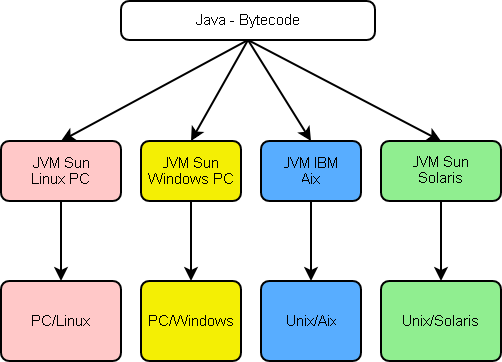
\includegraphics[width=1\linewidth]{./Java-jvm}
\caption[Java Virtual Machine als Schnittstelle]{Java Virtual Machine als Schnittstelle}
\label{fig:Java-jvm}
\end{figure}\newpage
Die JVM besteht aus folgenden Teilen:
\begin{itemize}
\item Classloader und Resolver
\item Garbage Collector
\item Execution Engine
\end{itemize}
\section{Funktionsweise}
Die Java Virtual Machine ist dazu da, um den Byte-Code der vom Java-Compiler erzeugt wurde, auf der jeweiligen Plattform auf der er ausgeführt werden soll ausführbar zu machen. Dazu werden die verschiedenen Byte-Code Dateien die erzeugt wurden (zu erkennen an Dateieindung "'class"') während der Laufzeit in die, vom jeweiligen Rechner verstandene Maschinensprache übersetzt. Die JVM arbeitet im Prinzip wie ein Interpreter, allerdings um einiges schneller, da nicht mehr auf Syntaxfehler geachtet werden muss. 
\section{Sicherheit}
Die JVM ist neben der Plattformunabhängigkeit auch für ein gewisses Maß an Sicherheit verantwortlich. Sie über wacht während der Laufzeit die Ausführung der Programme, verhindert Pufferüberläufe, welche zu unvorhersehbarem Verhalten wie zum Beispiel ein Absturz des Programmes führen können. Diese Überwachung ist allerdings ziemlich einfach, da Java Zeiger nur implizit unterstützt.
\section{Optimierungsverfahren}
Um die Performance von Java-Programmen zu erhöhen, setzen die meisten Java-VMs sogenannte JIT-Compiler (Just-In-Time-Compiler oder JITC) ein, die unmittelbar während des Programmablaufs den Bytecode "'genau zur rechten Zeit"' dauerhaft in Maschinensprache übersetzen. Eine Weiterentwicklung ist der Hotspot-Optimizer, welcher dynamische Optimierung anbietet.
\subsection{Dynamische Optimierung}
Oft ist zum Zeitpunkt der Kompilierung nicht bekannt, welche konkreten Eingaben eine Software verarbeiten muss. Demnach muss die Software mit allen Arten von Eingaben zurechtkommen. Die Eingabe wird deshalb in Variablen gespeichert. Nach dem Start des Programms werden jedoch viele Variablen nicht mehr geändert. Folglich sind diese - von einem Zeitpunkt kurz nach dem Start an - Konstanten. Wird nun erst nach diesem Zeitpunkt die Software für die System-Architektur kompiliert (dies ist bei Java Hotspot der Fall), so können diese Konstanten berücksichtigt werden. Bestimmte Verzweigungen, die nur von solchen „Halbkonstanten“ abhängig sind, sind dann für immer eindeutig und stellen somit kein Risiko für eine falsche Sprungvorhersage dar. Ein solcher Programmcode kann also schneller ablaufen als zu früh compilierter Code.
\subsection{Implementierung in Hardware}
Ausführungen in Hardware sind Java-Prozessoren, Mikroprozessoren, die Java-Bytecode als Maschinensprache verwenden. Sie konnten sich gegen die schnelle Steigerung der Leistungsfähigkeit von Standard-PC und JVM nicht durchsetzen.
\section{Threads}
Die Java VM schottet die in ihr laufenden Prozesse vom Betriebssystem ab (Green Threads). Sie bildet standardmäßig Java-Threads durch Threads des Betriebssystems ab. Nur in Ausnahmefällen erfolgt das Thread-Management durch die Java VM. Somit ist es auch möglich, auf einem Betriebssystem, das kein Multithreading unterstützt, eine Java VM mit vollem Funktionsumfang anzubieten.
Die Java VM hat stets volle und standardkonforme Kontrolle über die Java-Threads, d.h. der Programmierer braucht nicht die betriebssystemspezifischen Multi-Threading/Tasking/Processing-Eigenschaften zu berücksichtigen und kann sich stets auf die JRE verlassen. Nachteil ist, dass Probleme, die von einem Thread ausgehen, seitens des Betriebssystems dem gesamten Prozess zugeordnet werden. Gängige Betriebssysteme (wie zum Beispiel Linux, Windows) erlauben Kontrolle über diese „nativen“ Threads allenfalls über Software von Drittanbietern, wie beispielsweise die mit dem JDK mitgelieferte VisualVM. Standardwerkzeuge wie zum Beispiel der Windows Taskmanager zeigen Systemthreads jedoch nicht an.
\section{JVM kompatible Sprachen}
Neben Java gibt es auch andere Sprachen, die als Programmiersprachen für JVM-Programme benutzt werden können. Unter anderem folgende Sprachen können auf einer JVM laufen:
\begin{itemize}
\item Clojure, ein Lisp-Dialekt
\item Ceylon
\item Erjang, ein Erlang-Dialekt für die JVM
\item Free Pascal, das auch unter der JVM einen Großteil der Object-Pascal-Konstrukte unterstützt
\item Groovy, eine dynamisch typisierte Programmiersprache
\item JRuby, eine 100 % Ruby-kompatible Implementierung
\item Jython (früher: JPython), ist eine reine Java-Implementierung der Programmiersprache Python
\item Scala, eine Sprache, die Eigenschaften von Java mit funktionaler Programmierung vereint
\item Kotlin, eine 2011 vorgestellte Sprache von JetBrains
\end{itemize}
Auch gibt es eine Reihe von Skript-Sprachen, die von Java aus aufrufbar sind. Dazu gehört JavaScript (mittlerweile standardisiert als ECMAScript) mit dem "'Rhino"'-Interpreter (ein Mozilla-Projekt) sowie JavaFX als eine Skript-Sprache vor allem für grafische Elemente.\cite{jvmEin}\cite{jvmEin1}
\chapter{Die Bestandteile der Java Virtual Machine}
Wie zuvor bereits erwähnt besteht die JVM aus folgenden Teilen:
\begin{itemize}
\item Classloader und Resolver
\item Garbage Collector
\item Execution Engine
\end{itemize}
Auf diese wird in den folgenden Punkten genauer eingegangen.
\section{Classloader und Resolver}

\section{Garbage Collector}

\section{Execution Engine}

\section{Java Hotspot JVM}
\cite{jvmEin1}
\bibliography{ref}
\end{document}